\documentclass[a4paper]{scrreprt}
\usepackage{graphicx}
\usepackage{listings}
\usepackage{color}
\usepackage{hyperref}
\usepackage{makeidx}
\usepackage{bbm}
\usepackage[super]{nth}


\usepackage{xcolor}
\usepackage{caption}
\DeclareCaptionFont{white}{\color{white}}
\DeclareCaptionFormat{listing}{\colorbox{white}{\parbox{\textwidth}{#1#2#3}}}
\captionsetup[lstlisting]{format=listing}

\lstset{ %
  language=C++,                % the language of the code
  basicstyle=\normalsize\ttfamily,           % the size of the fonts that are used for the code
%   numbers=left,                   % where to put the line-numbers
%   numberstyle=\tiny\color{gray},  % the style that is used for the line-numbers
%   stepnumber=2,                   % the step between two line-numbers. If it's 1, each line 
%                                   % will be numbered
%   numbersep=5pt,                  % how far the line-numbers are from the code
%   backgroundcolor=\color{white},      % choose the background color. You must add \usepackage{color}
%   showspaces=false,               % show spaces adding particular underscores
%   showstringspaces=false,         % underline spaces within strings
%   showtabs=false,                 % show tabs within strings adding particular underscores
%   frame=single,                   % adds a frame around the code
%   rulecolor=\color{black},        % if not set, the frame-color may be changed on line-breaks within not-black text (e.g. commens (green here))
%   tabsize=2,                      % sets default tabsize to 2 spaces
%   captionpos=b,                   % sets the caption-position to bottom
%   breaklines=true,                % sets automatic line breaking
%   breakatwhitespace=false,        % sets if automatic breaks should only happen at whitespace
%   title=\lstname,                   % show the filename of files included with \lstinputlisting;
%                                   % also try caption instead of title
%   keywordstyle=\color{blue},          % keyword style
%   commentstyle=\color{dkgreen},       % comment style
%   stringstyle=\color{mauve},         % string literal style
%   escapeinside={\%*}{*)},            % if you want to add a comment within your code
%   morekeywords={*,...}               % if you want to add more keywords to the set
}

\usepackage{amsmath}
\usepackage{empheq}

\makeindex

\newcommand{\phFac}[1]{\mathrm{e}^{\mathrm{i} #1}}
\newcommand{\phFacneg}[1]{\mathrm{e}^{-\mathrm{i} #1}}
\newcommand{\planew}[2]{\mathrm{e}^{\mathrm{i} \mathbf{#1} \mathbf{#2}}}
\newcommand{\planewneg}[2]{\mathrm{e}^{-\mathrm{i} \mathbf{#1} \mathbf{#2}}}
\newcommand{\blf}[3]{\mathbf{#1}_{#2 \mathbf{#3}}}
\newcommand{\blfs}[3]{#1_{#2 \mathbf{#3}}}
\newcommand{\vp}[1]{\mathbf{#1}_{\mathcal{\parallel}}}
\newcommand{\ve}[1]{\mathbf{#1}}
\newcommand{\pd}[1]{\frac{\partial}{\partial #1}}
\newcommand{\scalProd}[2]{\langle #1 | #2 \rangle}
\newcommand{\bra}[1]{\langle #1 |}
\newcommand{\ket}[1]{|#1 \rangle}
\newcommand{\ann}[2]{#1^{\phantom{\dagger}}_{#2}}
\newcommand{\cre}[2]{#1^\dagger_{#2}}
\newcommand{\ud}{^{\phantom{\dagger}}}
\newcommand{\dd}{_{\phantom{\dagger}}}

\begin{document}

\title{Multigrid}
\subtitle{A highly versatile integration grid class for C++}
\author{Tobias Stollenwerk}
\maketitle

\tableofcontents

% % From now on put page enumeration into topline
% \pagestyle{headings}



%%%%%%%%%%%%%%%%%%%%%%%%%%%%%%%%%%%%%%%%%%%%%%%%%%%%%%%%%%%%%%%%%%%%%%%%%%%%%%%%%%%%%%%%%%%%%%%%%%%%%%%%%%%%%%%%%%%
%%%%%%%%%%%%%%%%%%%%%%%%%%%%%%%%%%%%%%%%%%%%%%%%%%%%%%%%%%%%%%%%%%%%%%%%%%%%%%%%%%%%%%%%%%%%%%%%%%%%%%%%%%%%%%%%%%%
%%%%%%%%%%%%%%%%%%%%%%%%%%%%%%%%%%%%%%%%%%%%%%%%%%%%%%%%%%%%%%%%%%%%%%%%%%%%%%%%%%%%%%%%%%%%%%%%%%%%%%%%%%%%%%%%%%%
%%%%%%%%%%%%%%%%%%%%%%%%%%%%%%%%%%%%%%%%%%%%%%%%%%%%%%%%%%%%%%%%%%%%%%%%%%%%%%%%%%%%%%%%%%%%%%%%%%%%%%%%%%%%%%%%%%%
%%%%%%%%%%%%%%%%%%%%%%%%%%%%%%%%%%%%%%%%%%%%%%%%%%%%%%%%%%%%%%%%%%%%%%%%%%%%%%%%%%%%%%%%%%%%%%%%%%%%%%%%%%%%%%%%%%%
%%%%%%%%%%%%%%%%%%%%%%%%%%%%%%%%%%%%%%%%%%%%%%%%%%%%%%%%%%%%%%%%%%%%%%%%%%%%%%%%%%%%%%%%%%%%%%%%%%%%%%%%%%%%%%%%%%%
%%%%%%%%%%%%%%%%%%%%%%%%%%%%%%%%%%%%%%%%%%%%%%%%%%%%%%%%%%%%%%%%%%%%%%%%%%%%%%%%%%%%%%%%%%%%%%%%%%%%%%%%%%%%%%%%%%%
\chapter{Introduction}

The multigrid class is a highly versatile integration grid class for \texttt{C++}. It features the integration of multiple grid regions in order to resolve sharp peaks or steps in the integrand function. Hereby one can choose between equidistant, tangential and logarithmically dense grid regions. Although the number of grid regions is not bounded, there is an index function which analytically calculates the inverse of the grid and is useful for fast interpolation purposes. Intersection and overlap of different grid region is possible will be dealt with by favouring the better resolve grid region.

The original purpose of the multigrid class was to resolve a lot of sharp Lorentz-like peaks in a self-consistent calculation on strongly correlated electron systems.


%%%%%%%%%%%%%%%%%%%%%%%%%%%%%%%%%%%%%%%%%%%%%%%%%%%%%%%%%%%%%%%%%%%%%%%%%%%%%%%%%%%%%%%%%%%%%%%%%%%%%%%%%%%%%%%%%%%
%%%%%%%%%%%%%%%%%%%%%%%%%%%%%%%%%%%%%%%%%%%%%%%%%%%%%%%%%%%%%%%%%%%%%%%%%%%%%%%%%%%%%%%%%%%%%%%%%%%%%%%%%%%%%%%%%%%
%%%%%%%%%%%%%%%%%%%%%%%%%%%%%%%%%%%%%%%%%%%%%%%%%%%%%%%%%%%%%%%%%%%%%%%%%%%%%%%%%%%%%%%%%%%%%%%%%%%%%%%%%%%%%%%%%%%
%%%%%%%%%%%%%%%%%%%%%%%%%%%%%%%%%%%%%%%%%%%%%%%%%%%%%%%%%%%%%%%%%%%%%%%%%%%%%%%%%%%%%%%%%%%%%%%%%%%%%%%%%%%%%%%%%%%
%%%%%%%%%%%%%%%%%%%%%%%%%%%%%%%%%%%%%%%%%%%%%%%%%%%%%%%%%%%%%%%%%%%%%%%%%%%%%%%%%%%%%%%%%%%%%%%%%%%%%%%%%%%%%%%%%%%
%%%%%%%%%%%%%%%%%%%%%%%%%%%%%%%%%%%%%%%%%%%%%%%%%%%%%%%%%%%%%%%%%%%%%%%%%%%%%%%%%%%%%%%%%%%%%%%%%%%%%%%%%%%%%%%%%%%
%%%%%%%%%%%%%%%%%%%%%%%%%%%%%%%%%%%%%%%%%%%%%%%%%%%%%%%%%%%%%%%%%%%%%%%%%%%%%%%%%%%%%%%%%%%%%%%%%%%%%%%%%%%%%%%%%%%
\chapter{Quick Start Guide}\label{chapter:quick_start_guide}
The purpose of this section is to give you a brief introduction of how the multigrid is used in practice. It may suffice for the most applications.

%%%%%%%%%%%%%%%%%%%%%%%%%%%%%%%%%%%%%%%%%%%%%%%%%%%%%%%%%%%%%%%%%%%%%%%%%%%%%%%%%%%%%%%%%%%%%%%%%%%%%%%%%%%%%%%%%%%
%%%%%%%%%%%%%%%%%%%%%%%%%%%%%%%%%%%%%%%%%%%%%%%%%%%%%%%%%%%%%%%%%%%%%%%%%%%%%%%%%%%%%%%%%%%%%%%%%%%%%%%%%%%%%%%%%%%
%%%%%%%%%%%%%%%%%%%%%%%%%%%%%%%%%%%%%%%%%%%%%%%%%%%%%%%%%%%%%%%%%%%%%%%%%%%%%%%%%%%%%%%%%%%%%%%%%%%%%%%%%%%%%%%%%%%
\section{Installation}
At the moment the only possibility to use the multigrid class is to directly incorporate the source file into your program. It is planned to create a library version. At first download the latest version of the multigrid class from
\begin{lstlisting}[language=bash]
https://github.com/tstollenw/multigrid
\end{lstlisting}
unpack it and put the files
\begin{lstlisting}
multigrid.cpp
multigrid.h
grid.cpp
grid.h
mesh.cpp
mesh.h
\end{lstlisting}
into your program directory. Include and link the files in the usual way. There is an example program \texttt{main.cpp} and the corresponding makefile \texttt{makefile} which will create an executable \texttt{example.out}. All examples used in this documentation are part of the example program and can be found in \texttt{main.cpp}.

%%%%%%%%%%%%%%%%%%%%%%%%%%%%%%%%%%%%%%%%%%%%%%%%%%%%%%%%%%%%%%%%%%%%%%%%%%%%%%%%%%%%%%%%%%%%%%%%%%%%%%%%%%%%%%%%%%%
%%%%%%%%%%%%%%%%%%%%%%%%%%%%%%%%%%%%%%%%%%%%%%%%%%%%%%%%%%%%%%%%%%%%%%%%%%%%%%%%%%%%%%%%%%%%%%%%%%%%%%%%%%%%%%%%%%%
%%%%%%%%%%%%%%%%%%%%%%%%%%%%%%%%%%%%%%%%%%%%%%%%%%%%%%%%%%%%%%%%%%%%%%%%%%%%%%%%%%%%%%%%%%%%%%%%%%%%%%%%%%%%%%%%%%%
\section{First Steps}\index{Grid}
The numerical calculation of an integral over some function $f(\omega)$
\begin{equation} \label{eqn:integral}
	I=\int d\omega f(\omega)
\end{equation}
can be written as
\begin{equation} \label{eqn:nintegral}
	I=\sum_{i=0}^M d\omega_i f(\omega_i)
\end{equation}
where the $\omega_i$ is the discrete integration grid and $d\omega_i$ are the corresponding weights. The integration grid is a mapping from a discrete index $i\in\{0,\dots,M\}$ to a continuous variable $\omega_i$. The multigrid class provides both the integration grid and its weights (which are calculated by the trapez rule) as well as an inverse mapping (back from any $\omega$ to the nearest index $i$).

In the following we will show the basic functionality of the multigrid class by some simple examples. All these examples are more or less all part of the example program \texttt{main.cpp}. At first we will create a simple equidistant grid with from $-4$ to $4$ with a resolution of $0.01$ by 

\vspace{1cm}
\noindent\begin{minipage}[l]{0.6\textwidth}
\begin{lstlisting}
multigrid mgrid;
mgrid.add_gr_equi(-4, 4, 0.01);
mgrid.create();
\end{lstlisting}
\end{minipage}
\begin{minipage}[]{0.4\textwidth}
	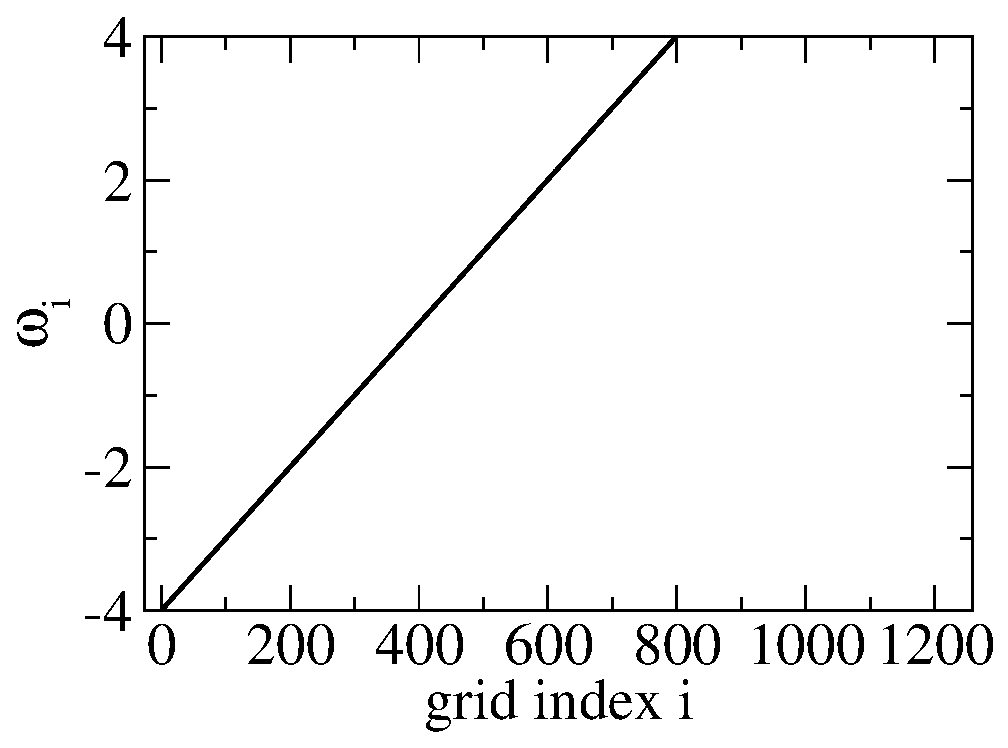
\includegraphics[width=1.0\textwidth]{pics/multigrid_00.eps}
\end{minipage}

\vspace{1cm}
After the declaration of the multigrid named \texttt{mgrid}, the member function \texttt{add\_gr\_equi} adds an equidistant grid region to the grid. The grid is created by invoking the \texttt{create} member function and it is accessed over its member variables (see table~\ref{tab:member}). 



\begin{table}[h]
	\begin{center}
		\begin{tabular}{l|l|l}\hline
		Name & Type & Description \\ \hline
		\texttt{M} & integer & Number of grid points\\\hline
		\texttt{omega} & STL-Vector & Grid (mapping $i\to\omega$ )\\\hline
		\texttt{domega} & STL-Vector & Weights of the grid\\\hline
		\texttt{omega\_min} & double & Minimum grid value (equal to \texttt{omega[0]}) \\\hline
		\texttt{omega\_max} & double & Maximum grid value (equal to \texttt{omega[M]}) \\\hline
		\texttt{inverse} & returns integer & Inverse mapping: $\omega\to i$ \\\hline
		\end{tabular}
	\end{center}
	\caption{Most important members of the multigrid}
	\label{tab:member}
\end{table}

The calculation of the above integral from $-4$ to $4$ is then done by

\begin{lstlisting}
double I=0;
for (int i=0; i<=mgrid.M; j++)
{
	I += f(mgrid.omega[i]) * mgrid.domega[i];
}
\end{lstlisting}

%%%%%%%%%%%%%%%%%%%%%%%%%%%%%%%%%%%%%%%%%%%%%%%%%%%%%%%%%%%%%%%%%%%%%%%%%%%%%%%%%%%%%%%%%%%%%%%%%%%%%%%%%%%%%%%%%%%
%%%%%%%%%%%%%%%%%%%%%%%%%%%%%%%%%%%%%%%%%%%%%%%%%%%%%%%%%%%%%%%%%%%%%%%%%%%%%%%%%%%%%%%%%%%%%%%%%%%%%%%%%%%%%%%%%%%
%%%%%%%%%%%%%%%%%%%%%%%%%%%%%%%%%%%%%%%%%%%%%%%%%%%%%%%%%%%%%%%%%%%%%%%%%%%%%%%%%%%%%%%%%%%%%%%%%%%%%%%%%%%%%%%%%%%
\section{Logarithmically Dense Grid Regions}\index{Grid region!logarithmic}
To resolve steps or very sharp peaks in the integrand function one needs a lot of integration grid points at specific regions. The multigrid class provides a tool to solve such problems: logarithmically dense grid regions (LGR). An LGR is determined by four variables, i.e.~the center of the grid region $\omega_0$ which corresponds for example to the position of a peak in the integrand function, the half width of the grid region $\omega_1$, the maximal resolution $d\omega_{max}$ at the center of the grid region and the minimal resolution $d\omega_{min}$ at the edges of the grid region (see figure~\ref{fig:lgr}). 
\begin{figure}[h]
	\centering
	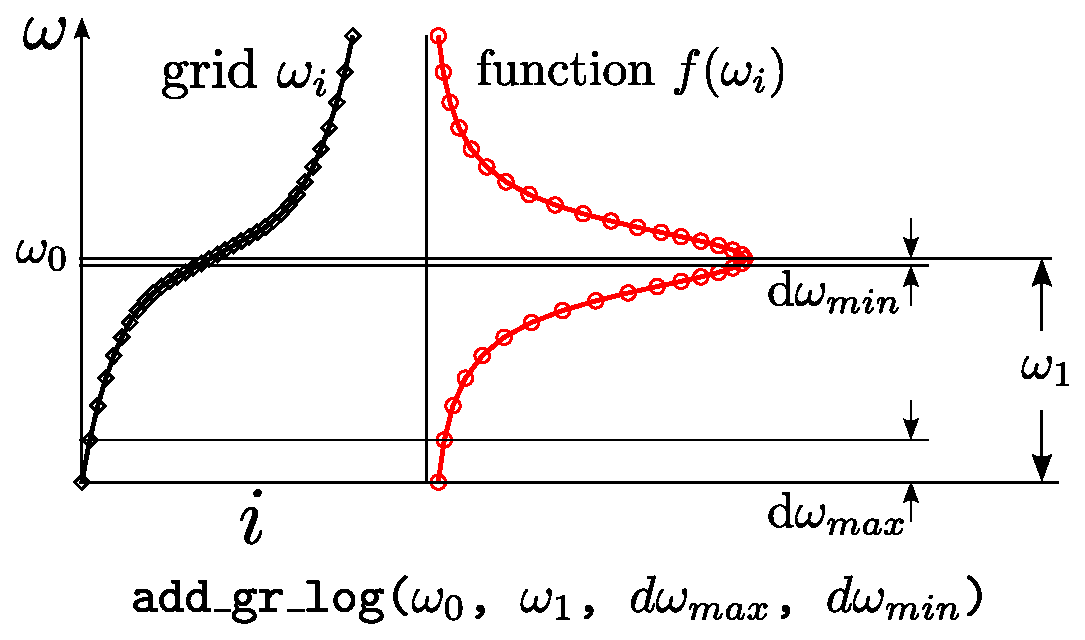
\includegraphics[width=0.6\textwidth]{pics/loggridregion.eps}
	\caption{Logarithmically dense grid region to resolve a peaked integrand function}
	\label{fig:lgr}
\end{figure}

It is created by the function \texttt{add\_gr\_log($\omega_0$, $\omega_1$, $d\omega_{max}$, $d\omega_{min}$)}. For example the following code adds a LGR on top of the equidistant grid region we used before. Note, that since the equidistant grid region was added first, it determines the outer boundaries of the whole grid (here from $-4$ to $4$). The first added grid region is therefore a special one and is called the basic grid region.
\\
\vspace{1cm}
\noindent\begin{minipage}[l]{0.6\textwidth}
\begin{lstlisting}
multigrid mgrid;
mgrid.add_gr_equi(-4, 4, 0.01);
mgrid.add_gr_log(0.3,0.5,0.001,0.01);
mgrid.create();
\end{lstlisting}
\end{minipage}
\begin{minipage}[]{0.4\textwidth}
	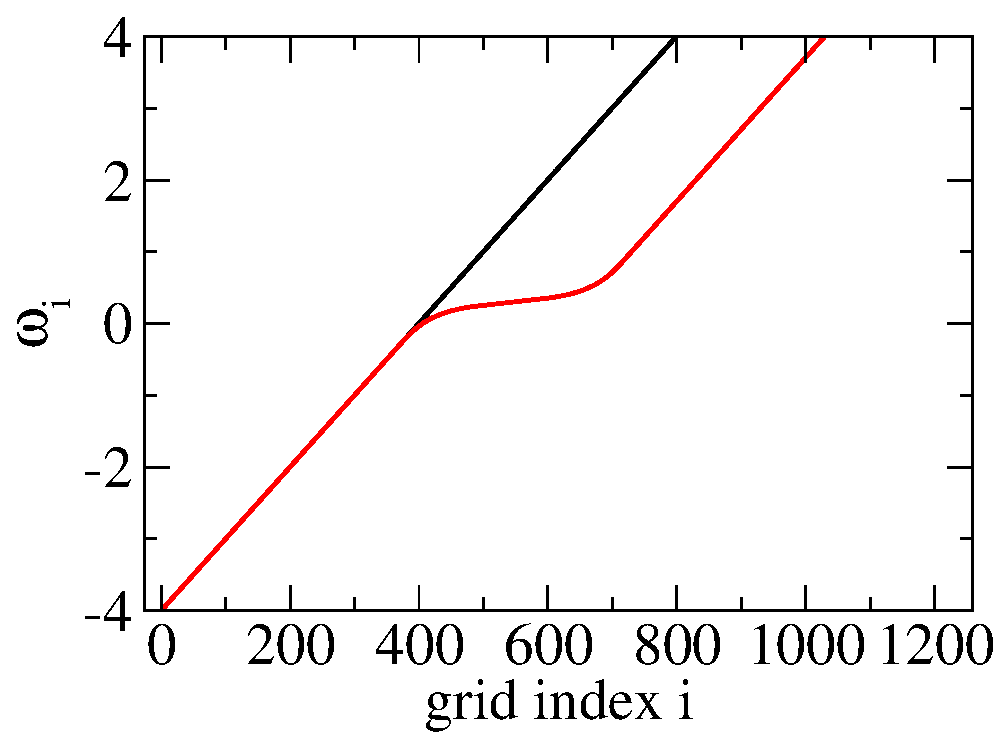
\includegraphics[width=1.0\textwidth]{pics/multigrid_01.eps}
\end{minipage}

The strength of the multigrid is that one can add now more and more grid regions on top of each other. The \texttt{create} function will take care of calculating intersection points between the grid regions by favoring the better resolved grid region. In the following example the there are two intersecting LGR on top of an equidistant grid region. 
\\
\vspace{1cm}
\noindent\begin{minipage}[l]{0.6\textwidth}
\begin{lstlisting}
multigrid mgrid;
mgrid.add_gr_equi(-4, 4, 0.01);
mgrid.add_gr_log(0.3,0.5,0.001,0.01);
mgrid.add_gr_log(0.6,0.5,0.001,0.01);
mgrid.create();
\end{lstlisting}
\end{minipage}
\begin{minipage}[]{0.4\textwidth}
	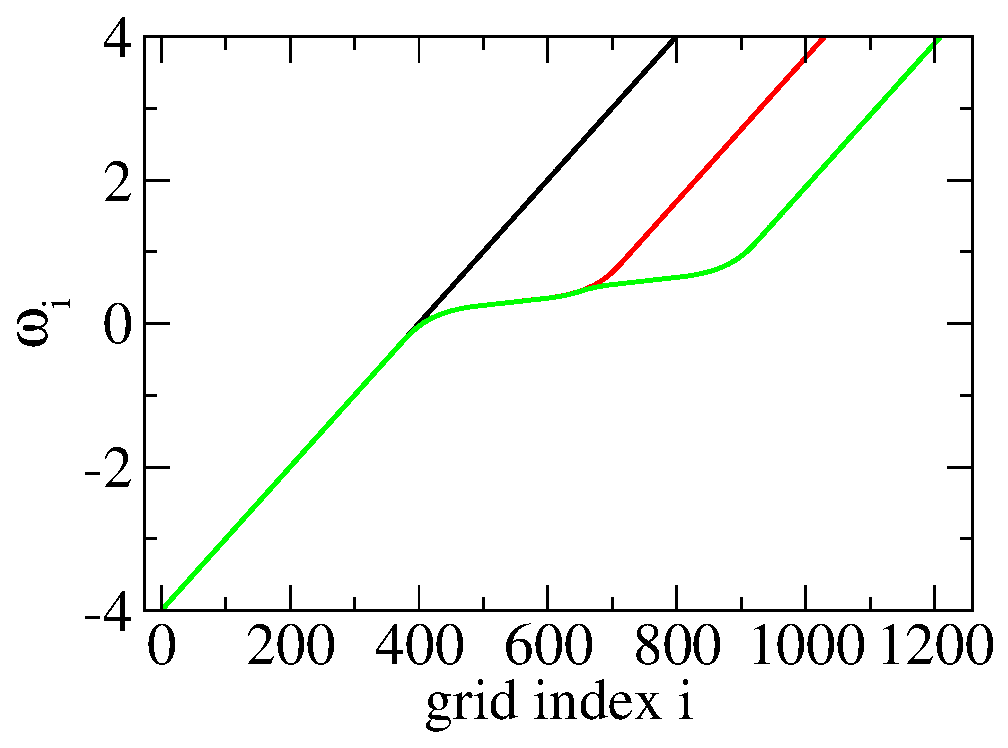
\includegraphics[width=1.0\textwidth]{pics/multigrid_02.eps}
\end{minipage}

These are only the basic features of the multigrid class. There is an algorithm which decides where to cut grid regions if there is overlap or even skip a particular grid region in special cases. The decisive element is the grid resolution exactly at the center of a given grid region. Hereby it is possible to add hundreds of grid regions on top of each other without losing the resolution at every single center point of the grid regions. In figure~\ref{fig:multiple_lgr} there is an example for the necessity for multiple LGR in the integration grid. The integrand function has several sharp peaks which have to be resolved. Each peak is resolved by a LGR.
\begin{figure}[h]
	\centering
	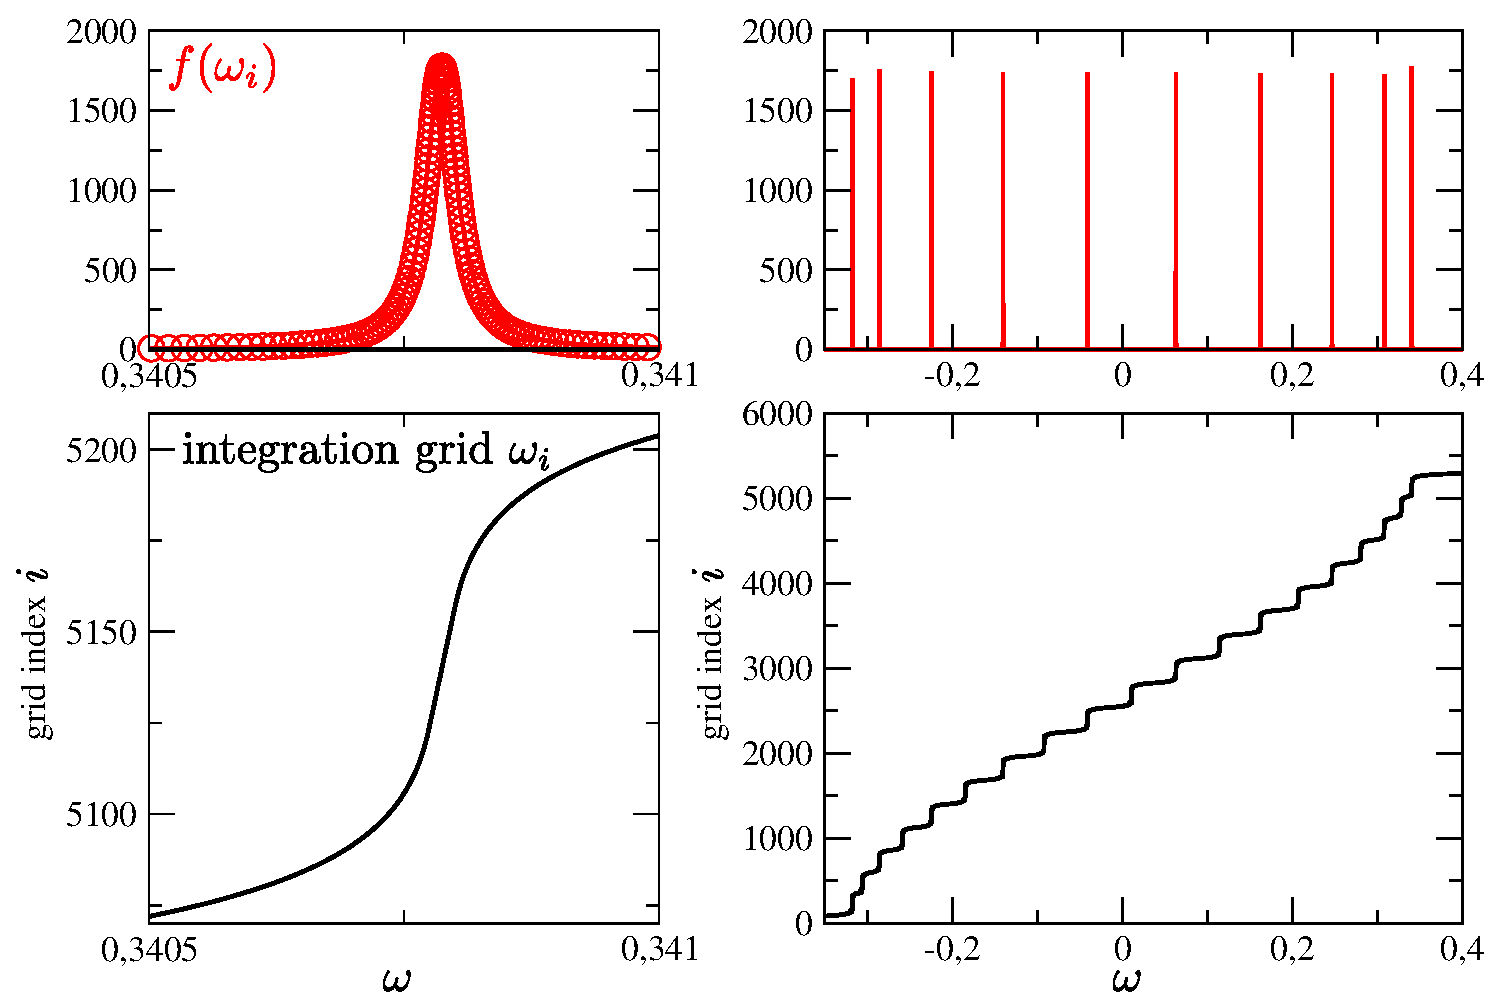
\includegraphics[width=0.9\textwidth]{pics/multiple_loggridregions.eps}
	\caption{Multigrid with various logarithmically dense grid regions to resolve a multiple peaked integrand function}
	\label{fig:multiple_lgr}
\end{figure}
\chapter{Numerical Integration}\label{chapter:numerical_integraion}
\section{Numerical Integration - Trapezoidal rule}
\index{Trapezoidal rule}
\index{Weights}
In this chapter, we will briefly review the concepts of numerical integration in one dimension. Consider integral over some function $f(\omega)$
\begin{equation}
	I=\int_a^b d\omega f(\omega)
\end{equation}
For numerical calculation one has to discretize the interval of integration $[a,b]$:
\[
	\omega \to \omega(i) \quad;\quad i\in\{0,\dots,M\}\quad\text{and}\quad \omega(0)=a,\quad \omega(M)=b.
\]
Where the strictly increasing mapping $\omega: \mathbbm{N} \to \mathbbm{R}: i \mapsto \omega(i)$ is called a grid. The numerical approximation for the integral now reads
\begin{equation} 
	I=\sum_{i=0}^M d\omega(i) f(\omega(i))
\end{equation}
where the $d\omega(i)$ are the so called weights. There are various methods to calculate the weights out of the grid itself. We will restrict ourselves to the trapezoidal rule which approximates the integrand function by linear regions connecting the sample points (see figure~\ref{fig:trapezoidal_rule}).
\begin{figure}[ht]
	\centering
	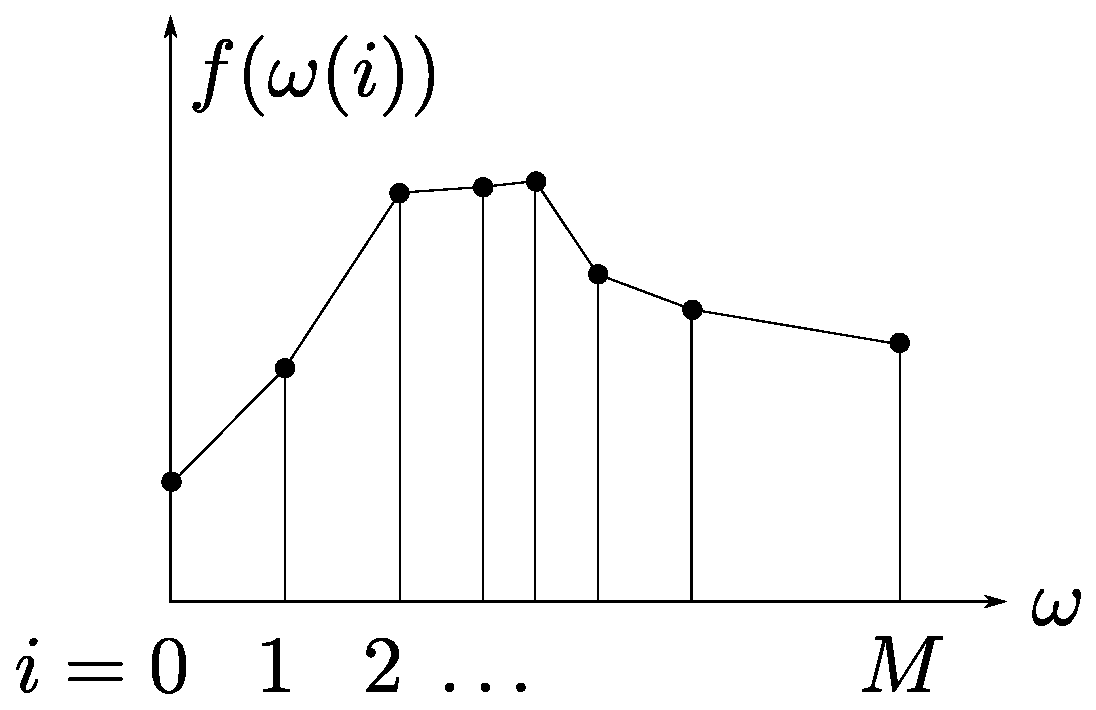
\includegraphics[width=0.3\textwidth]{pics/trapez.eps}
	\caption{Trapezoidal rule for a non-equidistant grid.}
	\label{fig:trapezoidal_rule}
\end{figure}

The numerical approximation for the integral is then
\begin{align*}
	I&=\sum_{i=0}^{M-1} \frac{f(\omega(i+1)) + f(\omega(i))}{2} (\omega(i+1)-\omega(i)) \\
	&=f_0\biggl( \underbrace{\frac{\omega(1)-\omega(0)}{2}}_{d\omega(0)}\biggr) + f_1 \biggl( \underbrace{\frac{\omega(N)-\omega(N-1)}{2}}_{d\omega(N)}\biggr) + \sum_{i=1}^{M-1} f(\omega(i)) \biggl( \underbrace{\frac{\omega(i+1)-\omega(i-1)}{2}}_{d\omega(i)}\biggr)\\
	&=\sum_{i=0}^{M} d\omega(i)\,f(\omega(i))
\end{align*}
therefore the weights are given by
\[
	d\omega(i)=\begin{cases}
		\frac{\omega(1)-\omega(0)}{2} \quad &i=0\\
		\frac{\omega(i+1)-\omega(i-1)}{2} \quad &i\in \{1,\dots,M-1\}  \\
		\frac{\omega(N)-\omega(N-1)}{2} \quad &i=M
	\end{cases}
\]

\section{Interpolation - Inverse mapping}\index{Interpolation}
\index{Inverse mapping}
In order to calculate a function $f$ which is known on a given grid $\omega(i)$, on another grid $\epsilon(i)$ we need to interpolate. We restrict ourselves to linear interpolation and we further assume, that the inverse mapping of the first grid
\[
	i(\omega):\;\mathbbm{R}\to\mathbbm{N}:\quad \omega \mapsto i\quad\quad;\;\omega\in[\omega(0), \omega(M)]
\]
is known.

The interpolation is then done in the following way. For each point of the new grid $\epsilon(j)\equiv \epsilon_j$ one calculates the inverse of the old grid $I=i(\epsilon_j)$. The corresponding old grid point $\omega(I)\equiv \omega_i$ is then the nearest grid point to the interpolation point $\epsilon_j$ (Figure~\ref{fig:interpolation}). 
\begin{figure}[ht]
	\centering
	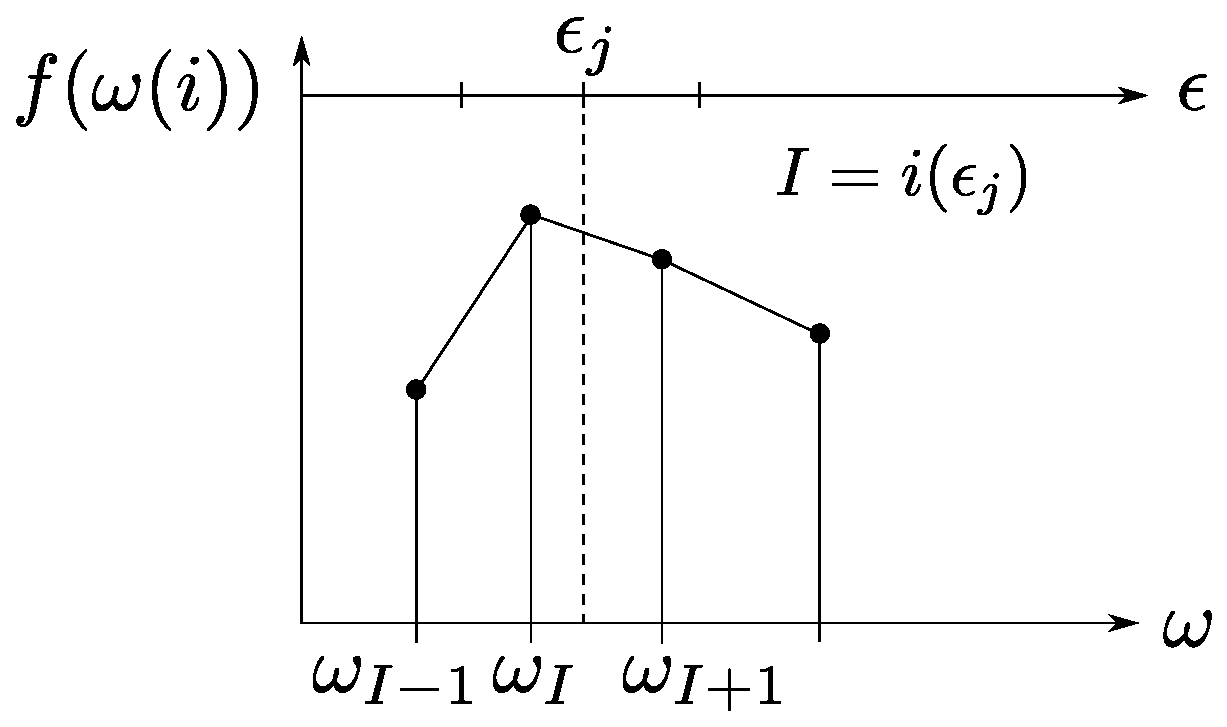
\includegraphics[width=0.4\textwidth]{pics/interpolation.eps}
	\caption{Linear interpolation of $f(\{\omega_i\})$ on a new grid $\{ \epsilon_j \}$}
	\label{fig:interpolation}
\end{figure}

The value of the function on the new grid $f(\epsilon_j)$ is then obtained by linear interpolation between the old grid point $\omega_I$ and its nearest neighbor (right neighbor for $\omega_I\leq\epsilon_j$, left neighbor for $\omega_I>\epsilon_j$).
\[
	f(\epsilon_j)=\begin{cases}
		f(\omega_I)+\frac{f(\omega_{I+1})-f(\omega_{I})}{\omega_{I+1}-\omega_{I}} (\epsilon_j-\omega_I) \quad \text{for } \omega_I<\epsilon_j \\
		f(\omega_I)+\frac{f(\omega_{I-1})-f(\omega_{I})}{\omega_{I-1}-\omega_{I}} (\epsilon_j-\omega_I) \quad \text{for } \omega_I>\epsilon_j 
	\end{cases}
\]







\chapter{Simple grids} \label{chapter:simple_grids}
In the following we will introduce all kinds of available grids together with their numerical structure. These grids will be the building blocks of the multigrid.
\section{The base class: grid}\index{Grid!class}
As it was shown in chapter \ref{chapter:numerical_integraion} all one needs for numerical integration is the integration grid itself and the corresponding weights. All of this is comprised in the class \texttt{grid} whose members are listed in table \ref{tab:member}. The grid class is defined in the \texttt{grid.h} file as follows

\begin{lstlisting}
class grid
{
        public:
        int M;
        double omega_min;
        double omega_max;
        vector <double> omega;
        vector <double> domega;
        virtual unsigned int inverse (double omega)=0;
};
\end{lstlisting}
The grid itself and its weights are \texttt{STL-vectors} \cite{stl}. The inverse mapping is virtual, and so is the grid class itself. Only the classes which are derived from the grid class are non-virtual. If one is not familiar with the concept of inheritance one can think of it in the following way: Since all integration grids should possess the above attributes (table \ref{tab:member}), it is reasonable to define a skeleton for an integration grid. This is the virtual grid class. It is not possible to create an instance of the grid class, but its possible to give it as an argument in a function. For example:
\begin{lstlisting}
void saveGrid(grid & mgrid, string filename)
{
        ofstream out;
        out.open(filename.c_str());
        for (int j=0; j!=mgrid.M+1; j++)
        {
                out << j << "\t" << mgrid.omega[j] << endl;
        }
        out.close();
}
\end{lstlisting}
This function can then take any kind of grid class (as long as it is derived from the basic grid class) as an argument. This is the whole purpose of using a virtual base grid class. In the following we will introduce all kinds of available grids.

\section{Equidistant grid: equigrid}\label{sec:equigrid}
\index{Grid!equidistant}
\index{equigrid}

The simplest grid class is the equidistant grid class. It is called \texttt{equigrid} and the grid is defined in the following way:
\[
	\omega(i) = \omega_{min} + d\omega \cdot i
\]
with $i\in {0,\dots,M}$ and $\omega(M)=\omega_{max}$. Beside the grid class attributes (table \ref{tab:member}), the equigrid has only one additional variable: the grid resolution $d\omega$. The inverse of $\omega(i)$ is given by
\[
	i(\omega)=\frac{\omega-\omega_{min}}{d\omega}
\]
The grid point density reads
\begin{equation}\label{eqn:equigrid_grid_point_density}
 \frac{di}{d\omega} (\omega) = \frac{1}{d\omega}
\end{equation}
The class is defined in the files \texttt{grid.h} and \texttt{grid.cpp}. Its defining member variable are listed in table \ref{tab:equigrid_defining_members}.
\begin{table}[h]
	\begin{center}
		\begin{tabular}{llp{3cm}l}
		Name            & Member                     & Constructor & Description           \\ 
		                &                            & Argument    &                       \\
		\hline
		$M$             & \texttt{int M}             & \nth{1}     & Number of grid points \\
		$\omega_{min}$  & \texttt{double omega\_min} & \nth{2}     & Lower boundary        \\
		$\omega_{max}$  & \texttt{double omega\_max} & \nth{3}     & Upper boundary        \\
		\end{tabular}
	\end{center}
	\caption{Defining properties of the \texttt{equigrid} class}
	\label{tab:equigrid_defining_members}
\end{table}
These are also the arguments of the equigrid constructor which is used for creating an instance of an equigrid:
\begin{lstlisting}
equigrid egrid(M, omega_min, omega_max);
\end{lstlisting}


\section{Tangential grid: tangrid}\label{sec:tangrid}
\index{Grid!tangential}
\index{tangrid}

The tangential grid is called \texttt{tangrid}. Beside the grid class attributes (table \ref{tab:member}), it has the a cluster point at $\omega_c$ \\

\begin{center}
	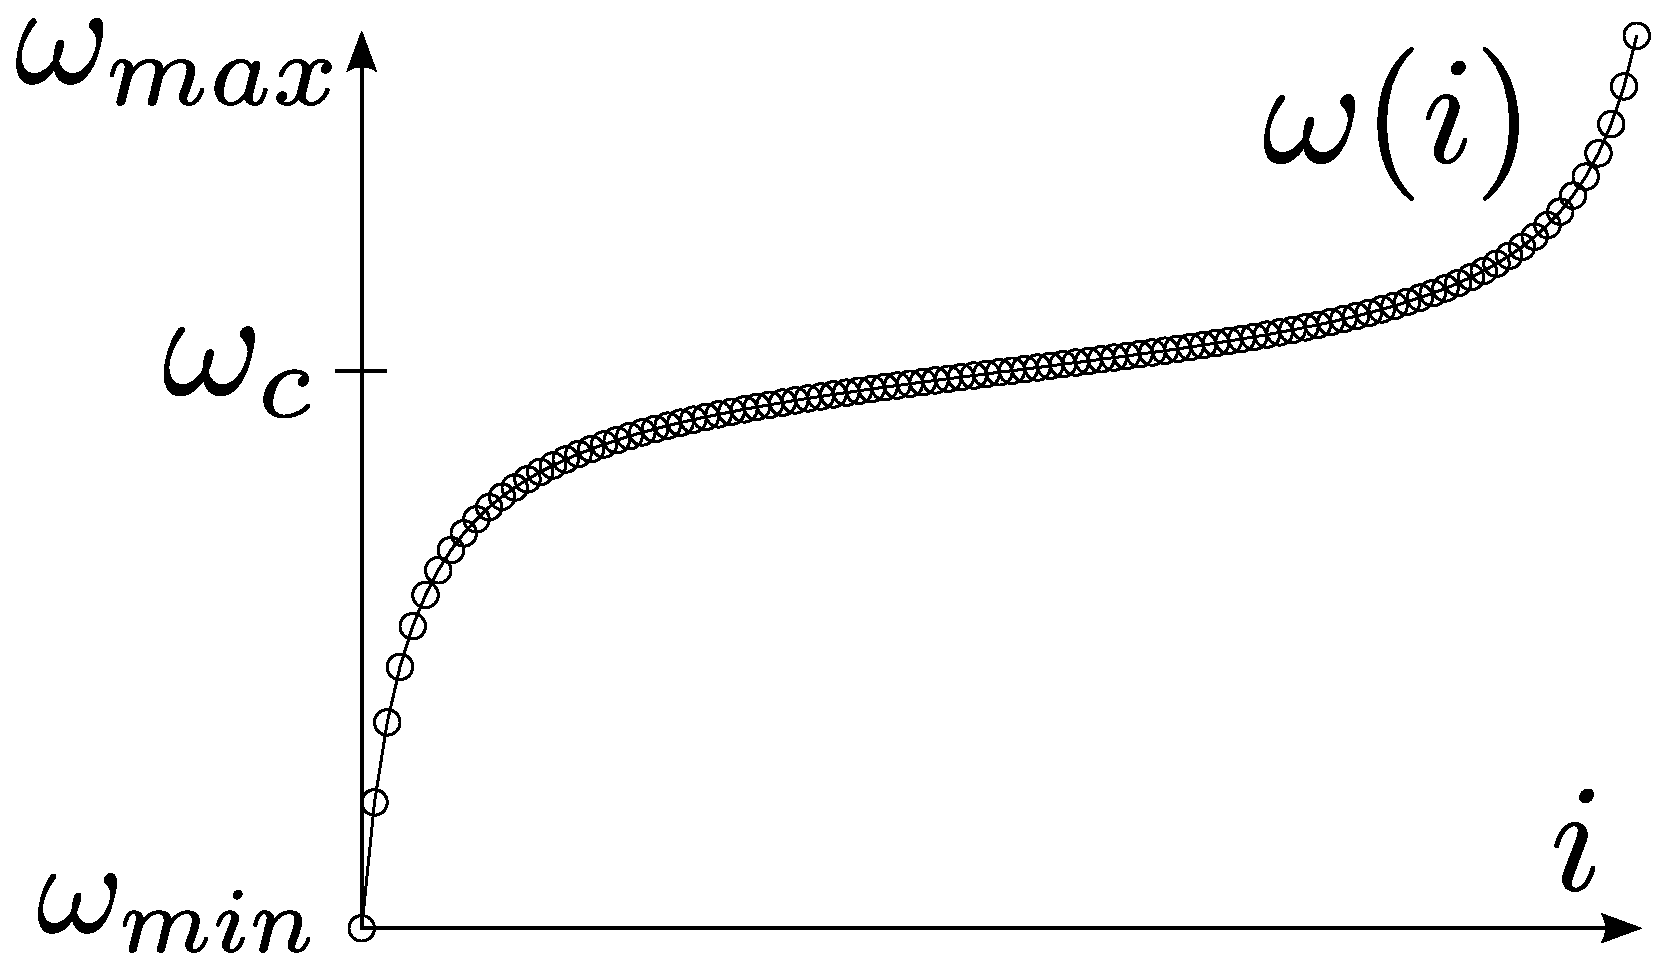
\includegraphics[width=0.3\textwidth]{pics/tangrid.eps}
\end{center}

\noindent The ``sharpness`` of this curve is controlled by the parameter $c$ and the grid is defined by
\[
	\omega(i)= c \tan (u_1+\Delta u \cdot i) + \omega_c
\]
where $i\in \{0,\dots,M\}$, and the parameters $u^0_1$ and $\Delta u$ are calculated such, that boundary conditions $\omega(0)=\omega_{min}$ and $\omega(M)=\omega_{max}$ are fulfilled. Hence
\begin{align*}
	u_1&=\arctan\left(\frac{\omega_{min}-\omega_c}{c}\right)\\
	u_2&=\arctan\left(\frac{\omega_{max}-\omega_c}{c}\right)\\
	\Delta u&=\frac{u_2-u_1}{M}
\end{align*}
The inverse of the grid is given by
\[
	i(\omega)=\frac{1}{\Delta u}\left(\arctan\left(\frac{\omega-\omega_c}{c}\right)-u_1\right)
\]
and the point density reads
\begin{equation}\label{eqn:tangrid_grid_point_density}
 \frac{di}{d\omega} (\omega) = \frac{1}{c \Delta u\left(1+\left(\frac{\omega-\omega_c}{c}\right)^2\right)}
\end{equation}

The class is defined in the files \texttt{grid.h} and \texttt{grid.cpp}. Its defining member variable are listed in table \ref{tab:tangrid_defining_members}.
\begin{table}[h]
	\begin{center}
		\begin{tabular}{llll}
		Name            & Member                     & Constructor & Description           \\ 
		                &                            & Argument    &                       \\ 
		\hline
		$M$             & \texttt{int M}             & \nth{1}     & Number of grid points \\
		$\omega_{min}$  & \texttt{double omega\_min} & \nth{2}     & Lower boundary        \\
		$\omega_{max}$  & \texttt{double omega\_max} & \nth{3}     & Upper boundary        \\
		$\omega_{c}$    & \texttt{double omega\_c}   & \nth{4}     & Center point          \\
		$c$             & \texttt{double c}          & \nth{5}     & Controls sharpness   \\
		\end{tabular}
	\end{center}
	\caption{Defining properties of the \texttt{tangrid} class}
	\label{tab:tangrid_defining_members}
\end{table}
These are also the arguments of the tangrid constructor which is used for creating an instance of a tangrid:
\begin{lstlisting}
tangrid tgrid(M, omega_min, omega_max, omega_c, c);
\end{lstlisting}

\section{Logarithmic grid: loggrid}\label{sec:loggrid}
\index{Grid!logarithmic}
\index{loggrid}
To resolve very sharp peaks in the integrand function the logarithmic grid is the right tool. It is named \texttt{loggrid} and it is constructed in the following way. There are three grid regions: one below I, one around II and one above III the center point $\omega_k$, which is the point with the highest grid point density.\\

\begin{center}
	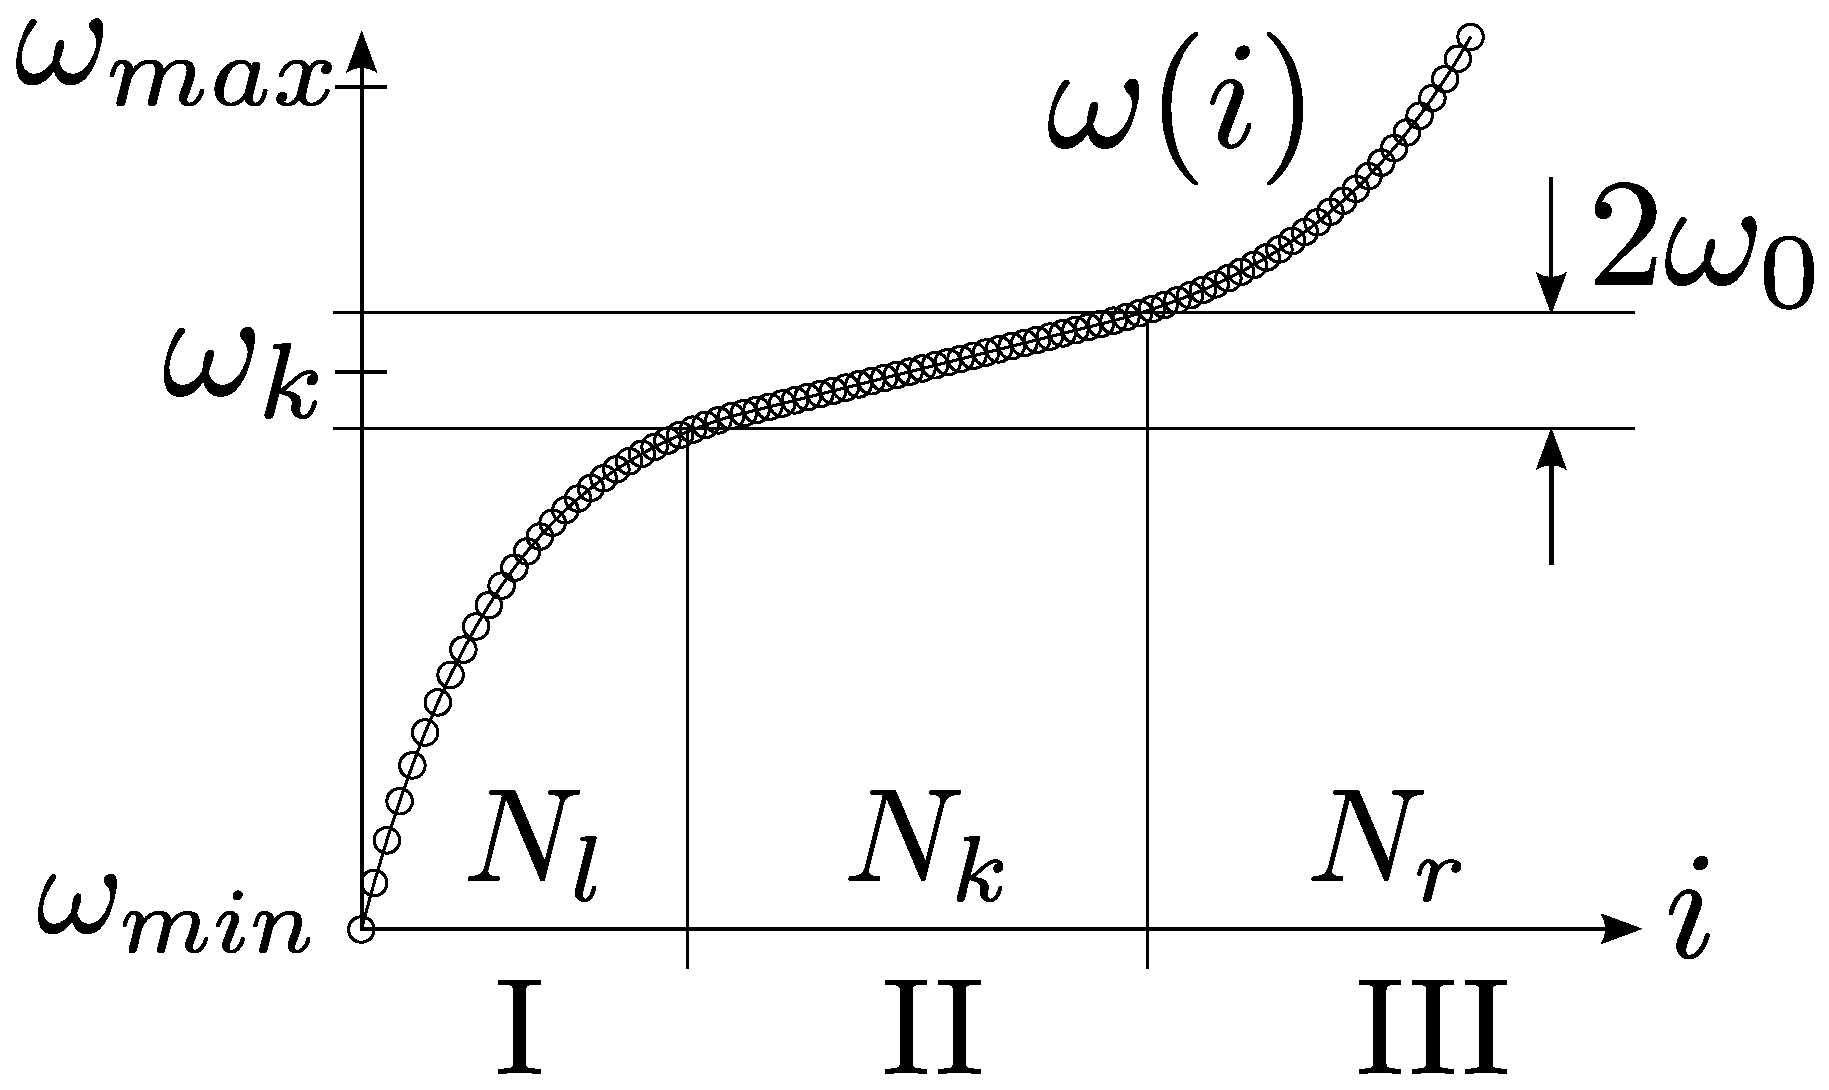
\includegraphics[width=0.4\textwidth]{pics/loggrid.eps}
\end{center}

Region I and III are exponential and region II is linear. The half width of the linear region $\omega_0$ also controls the ''sharpness`` of the exponential grid regions. The number of grid points in region I, $N_l$ and in region III, $N_r$ can be chosen different from each other. Both will also influence the ''sharpness'' of the exponential grid regions. The resolution of the linear grid region $d\omega_k$ is the same as the maximal resolution in the exponential grid regions and it determines the number of grid points in region II, $N_k$ (see Appendix \ref{sec:app_loggrid_max_resolution}). The grid is defined as
\begin{equation}\label{eqn:loggrid_definition}
	\omega(i)=\begin{cases}
		-\exp(-c_1(i-i_1)) + \omega_k 		\quad & i\in\{0,\dots,N_l-1\} \\ 
		\omega_k-\omega_0+d\omega_k(i-N_l)	\quad & i\in\{N_l,\dots,N_l+N_k-1\} \\ 
		\exp(c_2(i-i_2-N_l-N_k)) + \omega_k 	\quad & i\in\{N_l+N_k,\dots,N_l+N_k+N_r\}
	\end{cases}
\end{equation}
The four boundary conditions:
\begin{align}\label{eqn:loggrid_boundary_conditions}
	\omega(0)&=\omega_{min} \quad &\omega(N_l-1)&=\omega_k-\omega_0 \notag \\
	\omega(N_l+N_k)&=\omega_k+\omega_0 \quad &\omega(N_l+N_k+N_r)&=\omega_{max}
\end{align}
determine the four parameters $i_1$, $i_2$, $c_1$ and $c_2$ (see Appendix \ref{sec:app_loggrid_boundary}). The inverse is given by
\[
	i(\omega)=\begin{cases}
		\frac{\log(\omega_k-\omega)}{-c_1} + i_1 \quad &\text{for } \omega\in[\omega_{min},\omega_k-\omega_0) \\
		\frac{\omega-\omega_k+\omega_0)}{d\omega_k} + N_l \quad &\text{for } \omega\in[\omega_k-\omega_0,\omega_k+\omega_0) \\
		\frac{\log(\omega-\omega_k)}{c_2} + i_2 + N_l + N_k \quad &\text{for } \omega\in[\omega_k+\omega_0, \omega_{max}]
	\end{cases}
\]
and the grid point density reads
\begin{equation}\label{eqn:loggrid_grid_point_density}
	\frac{di(\omega)}{d\omega}=\begin{cases}
		\frac{1}{c_1(\omega_k-\omega)} \quad &\text{for } \omega\in[\omega_{min},\omega_k-\omega_0) \\
		\frac{1}{d\omega_k} \quad &\text{for } \omega\in[\omega_k-\omega_0,\omega_k+\omega_0) \\
		\frac{1}{c_2(\omega-\omega_k)}  \quad &\text{for } \omega\in[\omega_k+\omega_0, \omega_{max}]
	\end{cases}
\end{equation}

The class is defined in the files \texttt{grid.h} and \texttt{grid.cpp}. Its defining member variable are listed in table \ref{tab:loggrid_defining_members}.
\begin{table}[h]
	\begin{center}
		\begin{tabular}{llll}
		Name            & Member                     & Constructor          & Description                         \\ 
		                &                            & Argument             &                                     \\ 
		\hline
		$N_l$           & \texttt{int N\_l}          & \nth{1}              & Number of grid points in region I   \\
		$N_r$           & \texttt{int N\_r}          & \nth{2}              & Number of grid points in region III \\
		$\omega_{min}$  & \texttt{double omega\_min} & \nth{3}              & Lower boundary                      \\
		$\omega_{max}$  & \texttt{double omega\_max} & \nth{4}              & Upper boundary                      \\
		$\omega_{k}$    & \texttt{double omega\_k}   & \nth{5}              & Center point                        \\
		$\omega_{0}$    & \texttt{double omega\_0}   & \nth{6}              & Half width of the region II         \\
		\end{tabular}
	\end{center}
	\caption{Defining properties of the \texttt{loggrid} class}
	\label{tab:loggrid_defining_members}
\end{table}
These are also the arguments of the loggrid constructor which is used for creating an instance of a loggrid:
\begin{lstlisting}
loggrid loggrid(N_l, N_r, omega_min, omega_max, omega_k, omega_0);
\end{lstlisting}

\section{Using the grid classes}\label{sec:using_the_grid_classes}
\index{equigrid}
\index{tangrid}
\index{loggrid}

All of the above grids are derived from the base class \texttt{grid}. Therefore it is possible to write an function which performs the numerical integration without specifying the type of grid one wants to use
\begin{lstlisting}
double integrate(double (&f)(double), grid & g)
{
	double I=0
	for (int i=0; i<=mgrid.M; i++)
	{
		I+= f(mgrid.omega[i]) * domega[i];
	}
	return I;
} 
\end{lstlisting}
which can then be used for example with an equigrid and a Gauss function
\begin{lstlisting}
double gauss(double x)
{
	return exp(-x*x);
}
int main()
{
        equigrid agrid(100, -4, 4);
        //tangrid agrid(100, -4, 4, 1, 0.5);
        //loggrid agrid(30, 30, -4, 4, 1, 0.4);
        double I=integrate(gauss, agrid);
}
\end{lstlisting}
But one can also change the comments in the code in such a way, that a tangrid or a loggrid is used for the integration of a Gauss function.




\chapter{Multigrid} \label{chapter:multigrid}
\index{Multigrid}
\section{Overview}
A multigrid consist of a single basic grid which defines the outer boundaries of the multigrid and multiple grid regions (GR). Each of these grid regions can be equidistant, tangential or logarithmic. If the grid regions overlap each other, they will be cut in such a way, that the grid resolution remains constant while crossing over the cutting point. It could also happen that a particular grid region is forced out by another grid region because the purpose of the former one is already served by the latter one. The first added grid region defines the outer boundaries of the multigrid and it is excluded from the cutting procedure. It is called basic grid region (BGR).

A multigrid is created in the following way (see listing \ref{lst:create_multigrid_sketch}). First it has to be initialized. Afterwards one can add, replace and remove multiple grid regions on the multigrid. This will be explained in detail in section \ref{sec:grid_regions}. Finally the member function \texttt{create} in invoked. Hereby the cutting and selection procedure will be performed and the multigrid will be created. 
\begin{lstlisting}[caption={Creating a multigrid},	label={lst:create_multigrid_sketch}]
multigrid mgrid;
... 
... //add, replace and remove grid regions
...
mgrid.create()
\end{lstlisting}
The multigrid is also derived from the grid class and can therefore be used exactly in the same way then the other grids (see chapter \ref{sec:using_the_grid_classes})

\section{Grid regions}\label{sec:grid_regions}
\index{Grid region}
In this chapter we will introduce the notion of a grid region. We will assume, that the purpose of a grid region is to resolve some feature of the integrand function which is located a a single point. This will be the center point of the grid region $\omega_c$. Together with the left and right boundaries $\omega_l$ and $\omega_r$, the type of grid region (equidistant, tangential or logarithmic) and the grid region parameters (e.g. $\omega_k$ and $\omega_0$ for the loggrid) these are the defining properties of a grid region. The grid region is implemented as a class named \texttt{gridregion} and is defined in the file \texttt{multigrid.h}. Its defining member variables are shown in table \ref{tab:grid_region_defining_members}.
\begin{table}[h]
	\begin{center}
		\begin{tabular}{ll}
		Name & Description \\ 
		\hline
		$\omega_c$  & Center point \\
		$\omega_l$  & Lower boundary \\
		$\omega_r$  & Upper boundary \\
		\texttt{type}  & Type of grid region \\
		\texttt{id}  & Name of the grid region (optional) \\
		 & Grid region parameters (e.g. $\omega_k$ and $\omega_0$ for the loggrid) \\
		\end{tabular}
	\end{center}
	\caption{Defining properties of the grid region}
	\label{tab:grid_region_defining_members}
\end{table}

It obvious, that a possible cutting point can not be arbitrary narrow to the center point $\omega_c$. For example in the loggrid case, for numerical reasons at least three point of the exponential grid regions must survive in order to have a starting, an intermediate and an endpoint of the grid. Also the corresponding weights should not be smaller than the machine precision. Therefore one introduces a buffer region around $\omega_c$ which is defined by its upper and lower boundaries $\omega_+$ and $\omega_-$. In section \ref{sec:cutting_procedure} we will see, that in order to calculate the cutting point according to the grid point density (grid resolution) the maximal grid resolution on both sides of the center point $d\omega_{min}^l$ and $d\omega_{min}^r$ is necessary. Hereby we assume that the grid point density is monotonically increasing from the boundaries towards the center of the grid region. (This is true for all three kinds of grids from chapter \ref{chapter:simple_grids}). Table \ref{tab:grid_region_derived_members} shows the relevant derived properties of the grid region class, i.e. they are calculated directly out of the defining properties.
\begin{table}[h]
	\begin{center}
		\begin{tabular}{ll}
		Name & Description \\ 
		\hline
		$\omega_+$  & Upper boundary of the buffer region around $\omega_c$ \\
		$\omega_-$  & Lower boundary of the buffer region around $\omega_c$ \\
		$d\omega_{min}^l$  & Maximal resolution left to $\omega_c$ \\
		$d\omega_{min}^r$  & Maximal resolution right to $\omega_c$ \\
		\end{tabular}
	\end{center}
	\caption{Relevant derived properties of the grid region}
	\label{tab:grid_region_derived_members}
\end{table}

Note that there are actually more member variables. But since they we will never appear to the user will not discuss them here. In the following we will introduce the different kinds of grid regions. There are equidistant, tangential and logarithmic grid regions. Naturally, the boundaries of a particular grid region $\omega_l$ and $\omega_r$ will correspond to the boundary $\omega_{min}$ and $\omega_{max}$ of the simple grids from chapter \ref{chapter:simple_grids}. In table \ref{tab:grid_region_types} the mapping from the grid class member variables to the grid region member variables is shown. As mentioned earlier, the boundaries of the buffer region around the center point are chosen such, that there will be 3 points left. In the case of the logarithmic grid region, the buffer region always includes the linear region II of the loggrid.
\begin{table}[h]
	\begin{center}
		\begin{tabular}{llll}
		Grid region & equidistant & tangential & logarithmic  \\ 
		variable    &             &            &              \\
		\hline 
		$\omega_c$    & -               & $\omega_c$     & $\omega_k$     \\
		$\omega_l$    & $\omega_{min}$  & $\omega_{min}$ & $\omega_{min}$ \\
		$\omega_r$    & $\omega_{max}$  & $\omega_{max}$ & $\omega_{max}$ \\
		\texttt{type} & \texttt{'equi'} & \texttt{'tan'} & \texttt{'log'} \\
		$\omega_+$         & $\omega_c+3d\omega$ & $\omega_c+3c\Delta u$ & $\omega(i=N_l+N_k+3)$ \\
		$\omega_-$         & $\omega_c-3d\omega$ & $\omega_c-3c\Delta u$ & $\omega(i=N_l-3)$  \\
		$d\omega_{min}^l$  & $d\omega$ & $c\Delta u$ & see Appendix \ref{sec:app_loggrid_max_resolution} \\
		$d\omega_{min}^r$  & $d\omega$ & $c\Delta u$ & see Appendix \ref{sec:app_loggrid_max_resolution} \\
		\end{tabular}
	\end{center}
	\caption{Relation of grid class and grid region member variables}
	\label{tab:grid_region_types}
\end{table}

\subsection{Adding grid regions}\label{subsec:grid_region_adding}
\index{Grid region!equidistant}
\index{Grid region!tangential}
\index{Grid region!logarithmic}
\index{Grid region!add}
In this section we introduce the syntax for adding grid regions to the multigrid. (See section \ref{subsec:grid_region_examples} for examples).
An equidistant grid region consists of an instance of an equigrid (see \ref{sec:equigrid}). It is added to the multigrid by the member function 
\begin{lstlisting}
void add_gr_equi
\end{lstlisting}
Its arguments are shown in table \ref{tab:add_gr_equi}.

\begin{table}[h]
	\begin{center}
		\begin{tabular}{lll}		
		Argument  & Type & Description \\ \hline
		\nth{1}   & \texttt{int}    & Number of grid points ($M$) \\ 
		\nth{2}   & \texttt{double} & Lower boundary ($\omega_l$) \\ 
		\nth{3}   & \texttt{double} & Upper boundary ($\omega_r$) \\ 
		\nth{4}   & \texttt{double} & Center point ($\omega_c$) \\ 
		(\nth{5}) & \texttt{string} & Name of the grid region (\texttt{id})(optional)\\ 
		\end{tabular}
	\end{center}
	\caption{Arguments of the member function \texttt{add\_gr\_equi}}
	\label{tab:add_gr_equi}
\end{table}

A tangential grid region consists of an instance of an tangrid (see \ref{sec:tangrid}). It is added to the multigrid by the member function 
\begin{lstlisting}
void add_gr_tan
\end{lstlisting}
Its arguments are shown in table \ref{tab:add_gr_tan}.

\begin{table}[h]
	\begin{center}
		\begin{tabular}{lll}		
		Argument  & Type & Description \\ \hline
		\nth{1}   & \texttt{int}    & Number of grid points ($M$) \\ 
		\nth{2}   & \texttt{double} & Lower boundary ($\omega_l$) \\ 
		\nth{3}   & \texttt{double} & Upper boundary ($\omega_r$) \\ 
		\nth{4}   & \texttt{double} & Center point ($\omega_c$) \\ 
		\nth{5}   & \texttt{double} & Controls sharpness ($c$) \\ 
		(\nth{6}) & \texttt{string} & Name of the grid region (\texttt{id})(optional)\\ 
		\end{tabular}
	\end{center}
	\caption{Arguments of the member function \texttt{add\_gr\_tan}}
	\label{tab:add_gr_tan}
\end{table}

A logarithmic grid region consists of an instance of an loggrid (see \ref{sec:loggrid}). It is added to the multigrid by the member function 
\begin{lstlisting}
void add_gr_log
\end{lstlisting}
Its arguments are shown in table \ref{tab:add_gr_log}.

\begin{table}[h]
	\begin{center}
		\begin{tabular}{lll}		
		Argument  & Type & Description \\ \hline
		\nth{1}   & \texttt{int}    & Number of grid points in region I ($N_l$) \\ 
		\nth{2}   & \texttt{int}    & Number of grid points in region III ($N_r$) \\ 
		\nth{3}   & \texttt{double} & Lower boundary ($\omega_l$) \\ 
		\nth{4}   & \texttt{double} & Upper boundary ($\omega_r$) \\ 
		\nth{5}   & \texttt{double} & Center point ($\omega_k$) \\ 
		\nth{6}   & \texttt{double} & Half width of region II ($\omega_0$) \\ 
		(\nth{7}) & \texttt{string} & Name of the grid region (\texttt{id})(optional)\\ 
		\end{tabular}
	\end{center}
	\caption{Arguments of the member function \texttt{add\_gr\_log}}
	\label{tab:add_gr_log}
\end{table}

\subsection{Replacing and removing grid regions}\label{subsec:grid_region_replace_remove}
\index{Grid region!equidistant}
\index{Grid region!tangential}
\index{Grid region!logarithmic}
\index{Grid region!replace}
\index{Grid region!remove}
We have seen, that if a grid region is added to the multigrid, it is optional give a name to this grid region. In contrast to that, you can only replace or remove grid regions which have a name. One can check if a grid region with the name \texttt{id} exists, by calling the function
\begin{lstlisting}
bool gr_exists(string id)
\end{lstlisting}
If this is the case one can remove it by
\begin{lstlisting}
void rem_gr(string id)
\end{lstlisting}
In order to replace a grid region by one with the same name but different attributes one calls one of the replace functions
\begin{lstlisting}
void replace_gr_equi(...)
void replace_gr_tan(...)
void replace_gr_log(...)
\end{lstlisting}
where the arguments are exactly the same as the one for the add functions for the corresponding type of grid (see tables \ref{tab:add_gr_equi}, \ref{tab:add_gr_tan} and \ref{tab:add_gr_log}). The only difference is that for the replace functions, you definitely have to give the name of the grid region which is to be replaced, as the \texttt{id} argument.

\subsection{Examples}\label{subsec:grid_region_examples}
\index{Grid region!add}
\index{Grid region!remove}
\index{Grid region!replace}

In this section we will show in some examples how the above grid regions can be added, replaced or removed from the multigrid. 

\begin{lstlisting}[caption={Example for the adding of equidistant grid regions},label={lst:add_gr_equi}]
multigrid mgrid;
mgrid.add_gr_equi(100, -1, 1, 0);
mgrid.add_gr_tan(100, 0.2, 0.5, 0.3, 0.01);
mgrid.add_gr_log(100, 100, 0.4, 0.7, 0.6, 1E-6, "lgrid");
mgrid.create()
\end{lstlisting}

In listing \ref{lst:add_gr_equi} we show an example for the adding of grid regions. At first an equidistant grid with $100$ points from $-4$ to $4$ is added to the multigrid. This defines the basic grid region and therefore the boundaries of the multigrid. The center point of a basic grid region (here at $0$) is obsolete because there is no cutting. Afterwards a tangential grid region with $200$ points from $0.2$ to $0.5$ with a center point at $0.3$ is added. The parameter $c$ is $0.01$ here. Finally a third, logarithmic grid region is added. It overlaps with the tangential grid region and an appropriate cutting point will be calculated such that the grid resolution remains constant across the cutting point. The logarithmic grid region is named   ``lgrid'' and has 100 points in both of the exponetial grid regions. Its boundaries are from $0.4$ to $0.7$, its center point $\omega_k$ is at $0.6$ and the half width of the linear region $\omega_0$ is $10^{-6}$.





\section{Cutting procedure}\label{sec:cutting_procedure}
\index{Cutting procedure}
If two grid regions intersect, they have to be cut or one of the grid regions has to be erased. This is the content of this chapter. 

\section{Subgrid and inserting grid regions}\label{sec:subgrids_and_insert}
\index{Subgrid}
\index{Inverse of the multigrid}
If all grid regions have gone through the cutting procedure explained in \ref{sec:cutting_procedure}, we are left with a bunch of non-intersection grid regions. These grid regions are now ready to be inserted into the basic grid region. But there is one difficulty we have not mentioned so far which is the fact that one has to take care of the inverse. Since all grid regions consist of one of the simple grid classes from chapter \ref{chapter:simple_grids}, their inverse mapping is know.

\section{Inverse of the multigrid}\label{sec:inverse_of_the_multigrid}
\index{Inverse of the multigrid}




\section{Fundamental and special grid regions}\label{sec:fundamental_and_special_grid_regions}
\index{Fundamental grid regions}
\index{Special grid regions}
\chapter{Mesh - Multigrid without Inverse Mapping}
There might be occasions where the inverse mapping of the multigrid is not needed. The mesh grid class is exactly the same as the multigrid class, but without the inverse mapping. All multigrid commands also work for the mesh class. For example 
\begin{lstlisting}
	mesh mgrid;
	mgrid.add_gr_equi(100, -1, 1, 0);
	mgrid.add_gr_tan(100, 0.2, 0.5, 0.3, 0.01);
	mgrid.add_gr_log(100, 100, 0.4, 0.7, 0.6, 1E-6, "gr");
	mgrid.add_sgr_equi(0.5, 0.8, 0.001);
	mgrid.create();
\end{lstlisting}
is exactly the same as listing \ref{lst:add_sgr}, except for the first line. Note that the mesh class is not optimized for fast initialization since internally, the mesh \texttt{create} function will call the multigrid \texttt{create} function, which takes care of all the subgrid indices needed for the inverse mapping.

In comparison to the multigrid, there are only two additional features, which at the same time destroys the possibility of calculating the inverse of a mesh. The first one is the adding of single points inside grid by
\texttt{add\_spoint}. The second one is the adding of terminating points which serve as the total upper and lower boundary of the mesh by \texttt{add\_lendpoint} for the lower endpoint and \texttt{add\_rendpoint} for the upper endpoint. Hereby it is possible to cut of a multigrid at arbitrary points for the prize of giving up the possibility of calculating an inverse mapping. Listing \ref{lst:mesh} shows an example for an instance of the mesh class.
\begin{lstlisting}[caption={Example of a mesh},label={lst:mesh}]
mesh amesh;
amesh.add_gr_equi(10, 0.0, 1, 0.5);
amesh.add_gr_log(0.75, 0.1, 1E-1, 1E-2);
amesh.add_spoint(0.76);
for (int j=0; j!=100; j++)
{
	amesh.add_spoint(0.6+j/100.0);
}
amesh.add_lendpoint(0.15);
amesh.add_rendpoint(0.85);
amesh.create();
\end{lstlisting}
Note, that a inserted points will always take care of not letting the grid point difference ($\sim$ weights) getting to small (beyond machine precision). This is achieved by skipping all existing points which are to narrow to the inserted point.
\appendix
\chapter{Loggrid parameter}
\section{Boundary conditions}
\label{sec:app_loggrid_boundary}
In the following we will show how the four boundary conditions (\ref{eqn:loggrid_boundary_conditions})
\begin{align}
	\omega(0)&=\omega_{min}   \label{eqn:loggrid_boundary_condition_1}\\
	\omega(N_l-1)&=\omega_k-\omega_0  \label{eqn:loggrid_boundary_condition_2}\\
	\omega(N_l+N_k)&=\omega_k+\omega_0   \label{eqn:loggrid_boundary_condition_3}\\
	\omega(N_l+N_k+N_r)&=\omega_{max}   \label{eqn:loggrid_boundary_condition_4}
\end{align}
determine the four parameters $i_1$, $i_2$, $c_1$ and $c_2$ in the definition of the logarithmic grid~(\ref{eqn:loggrid_definition}):
\begin{equation*}
	\omega(i)=\begin{cases}
		-\exp(-c_1(i-i_1)) + \omega_k 		\quad & i\in\{0,\dots,N_l-1\} \\ 
		\omega_k-\omega_0+d\omega_k(i-N_l)	\quad & i\in\{N_l,\dots,N_l+N_k-1\} \\ 
		\exp(c_2(i-i_2-N_l-N_k)) + \omega_k 	\quad & i\in\{N_l+N_k,\dots,N_l+N_k+N_r\}
	\end{cases}
\end{equation*}

\vspace{1cm}
\noindent\underline{Determine $i_1$ and $c_1$:}\\

\noindent Insert \ref{eqn:loggrid_definition} into (\ref{eqn:loggrid_boundary_condition_1}) and (\ref{eqn:loggrid_boundary_condition_2}):
\begin{align}
	-\exp(-c_1(0-i_1))+\omega_k&=\omega_{min} \quad \Leftrightarrow \quad \log(\omega_k-\omega_{min})=c_1 i_1 \label{eqn:app_loggrid_boundary_condition_1_1}\\
	-\exp(-c_1(N_l-1-i_1))+\omega_k&=\omega_k-\omega_0 \quad \Leftrightarrow \quad \log(\omega_0)=-c_1(N_l-1-i_1) \label{eqn:app_loggrid_boundary_condition_2_1}
\end{align}
Difference (\ref{eqn:app_loggrid_boundary_condition_1_1}) $-$ (\ref{eqn:app_loggrid_boundary_condition_2_1}):
\[
	\log\left(\frac{\omega_k-\omega_{min}}{\omega_0}\right)=c_1 (N_l-1) \quad \boxed{\Rightarrow c_1=\frac{\log\left(\frac{\omega_k-\omega_{min}}{\omega_0}\right)}{N_l-1}}
\]
Insert into (\ref{eqn:app_loggrid_boundary_condition_2_1}):
\[
	\boxed{i_1=\frac{\log(\omega_k-\omega_{min})}{c_1}}
\]

\newpage
\vspace{1cm}
\noindent\underline{Determine $i_2$ and $c_2$:}\\

\noindent Insert \ref{eqn:loggrid_definition} into (\ref{eqn:loggrid_boundary_condition_1}) and (\ref{eqn:loggrid_boundary_condition_2}):
\begin{align}
	\exp(c_2(0-i_2))+\omega_k&=\omega_k+\omega_0 \quad \Leftrightarrow \quad \log(\omega_0)=c_2 (0-i_2) \label{eqn:app_loggrid_boundary_condition_3_1}\\
	\exp(c_2(N_r-i_2))+\omega_k&=\omega_{\max} \quad \Leftrightarrow \quad \log(\omega_{max}-\omega_k)=c_2(N_r-i_2) \label{eqn:app_loggrid_boundary_condition_4_1}
\end{align}
Difference (\ref{eqn:app_loggrid_boundary_condition_4_1}) $-$ (\ref{eqn:app_loggrid_boundary_condition_3_1}):
\[
	\log\left(\frac{\omega_{max}-\omega_k}{\omega_0}\right)=c_2 (N_r)\\\Rightarrow \boxed{c_2=\frac{\log\left(\frac{\omega_{max}-\omega_k}{\omega_0}\right)}{N_r}}
\]
Insert into (\ref{eqn:app_loggrid_boundary_condition_4_1}):
\[
	\boxed{i_2=-\frac{\log(\omega_{max}-\omega_k)}{c_2} + N_r}
\]
\section{Maximal resolution}
\label{sec:app_loggrid_max_resolution}
The maximal resolution of the exponential grid regions to the left (region I), $d\omega_{min}^{l}$ and to the right (region III), $d\omega_{min}^{r}$ of the center point in a logarithmic grid reads
\begin{align*}
	d\omega_{min}^{l} & = \omega(N_l-1)-\omega(N_l-2) \notag \\
	& = -\exp(-c_1(N_l-1-i_1))+exp(-c_1(N_l-2-1_1)) \notag \\
	& = \exp(-c_1(N_l-1-i_1))(e^{c_1}-1)
\end{align*}
analogously we have
\begin{align*}
	d\omega_{min}^{r} & = \omega(N_l+N_k+1)-\omega(N_l+N_k) \notag \\
	& = \exp(-c_2 i_2)(e^{c_2}-1)
\end{align*}
The resolution of the linear grid (region II) will be the minimum of both
\[
	d\omega_k = min( d\omega_{min}^{l} ,\,d\omega_{min}^{r})
\]
\chapter{Calculation of cutting points}\label{chapter:app_cutting_points}
\index{Cutting points}







\bibliographystyle{ieeetr}
\addcontentsline{toc}{chapter}{\bibname}
\bibliography{multigrid_documentation}


\printindex

\end{document}

